\documentclass[11pt]{ctexart}
\usepackage{fontspec}
\usepackage{booktabs}
\usepackage{caption}
\usepackage{float}
\usepackage[left=1in, right=1in, top=1in, bottom=1in,headheight=0pt,headsep=0pt]{geometry}
\usepackage{amsmath, amssymb}
\usepackage{graphicx}
\usepackage{url}
\pagestyle{plain}
\usepackage{listings}
\lstset{
    basicstyle=\scriptsize\ttfamily,
    numbers=left,
    numberstyle=\scriptsize\ttfamily,
    breaklines=true,
    columns=fixed,       
    frame=tblr,
    morekeywords={write},           
}

\setmainfont{texgyrepagella-regular.otf} %  正文字体
% \setmonofont{IBM Plex Mono}
\setlength{\parskip}{1ex plus 0.5ex minus 0.2ex}
\bibliographystyle{elsarticle-num}

\title{线程同步机制——实验说明文档}
\author{刘佳玮,20031211496,计算机科学与技术学院}
\date{}

\newenvironment{note}{\kaishu 注:}{}

\begin{document}

\maketitle

\begin{abstract}
本次实验使用了互斥量、信号量、读写锁和条件变量共四项技术来保证{\ttfamily g\_Count}
结果的正确性,均得到了理想的试验结果。
    
若无特殊声明,这四组实验的所有程序基于C语言,均依赖{\ttfamily pthread.h}库,
编译方式均为{\ttfamily gcc -fopenmp filename.c}。
互斥量,信号量和条件变量的程序在编译后的执行方式为{\ttfamily ./a.out};
为方便结果分析,需要将读写锁的执行结果重定向输出至文件,因此
执行方式为{\ttfamily ./a.out > result.txt},所有代码和结果文件均
会提交。
\end{abstract}

\tableofcontents
\newpage

\section{电脑配置}

电脑基本配置如下所示:
\begin{enumerate}
    \item CPU:i7-9750H,6核12线程。
    \item RAM:32GB。
    \item GPU:UHD Graphics 630, 256MB。
    \item 操作系统:Manjaro 20.1.2 (基于Arch二次开发的linux发行版),内核:5.4.72-1。
\end{enumerate}

\section{互斥量}

\subsection{互斥量原理解析}

互斥量允许多个线程安全地共享一个关联的软件或者硬件资源。当一个线程想使用共享资源时,它必须先通过获取互斥量以获得专有的访问权限,成功加锁才能操作,操作结束解锁。
如果该互斥量已被另一个线程锁定,请求线程可以等待该互斥量被解锁。

因此同一时刻,只能有一个线程持有该锁。因为资源是共享的,线程间也还是竞争的,但通过锁就将资源的访问变成互斥操作,线程不能同时操作数据,所以能保证结果正确。
核心语法如下所示:
\begin{enumerate}
    \item {\ttfamily pthread\_mutex\_t lock;} 创建互斥锁;
    \item {\ttfamily pthread\_mutex\_init(\&lock, NULL);} 初始化互斥锁;
    \item {\ttfamily pthread\_mutex\_lock(\&lock);} 获取互斥锁;
    \item {\ttfamily pthread\_mutex\_unlock(\&lock);} 释放互斥锁;
    \item {\ttfamily pthread\_mutex\_destroy(\&lock);} 在不使用互斥锁后,销毁互斥锁。
\end{enumerate}

\begin{note}
    锁定互斥量后,线程可以长时间地安全地使用相关联的资源。但是单个线程持有互斥量时间应尽可能的短,
    避免其他线程一直处于等待状态。当线程不再需要使用资源时,它必须将互斥量解锁,使得其它线程可以使用该资源。
\end{note}

\subsection{互斥量实验流程与结果分析}

根据原理解析,在程序中只需要在{\ttfamily g\_Count++}前添加获取锁操作,在{\ttfamily g\_Count++}后添加释放锁的操作即可。
创建200个线程,在程序内设置循环10次运行互斥量的实验,并分别输出每次运行的结果,如图\ref{mutex}所示。对代码和结果进行分析可知,程序运行正确。代码见提交作业
中的{\ttfamily mutex.c}文件。
 
\begin{figure}[ht]
    \centering
    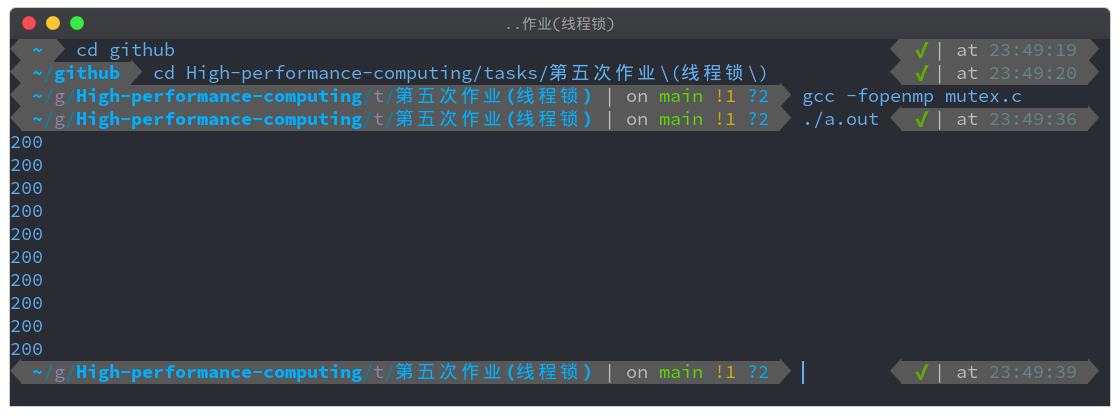
\includegraphics[scale=0.35]{../mutex.png}
    \caption{互斥量试验结果图}
    \label{mutex}
\end{figure}

\section{信号量}

\subsection{信号量原理解析}

首先,信号量的使用需要导入相关头文件:{\ttfamily \#include <semaphore.h>}。
信号量是一个同步对象,用于保持在0至指定最大值(初始化指定)之间的一个计数值,它只能被两个标准的原语{\ttfamily wait}和{\ttfamily post}来访问。

当线程访问共享资源时,需完成一次对信号量的等待{\ttfamily wait}操作,该计数值减一;
当线程访问完毕共享资源时,需要完成一次对信号量的释放{\ttfamily post}操作,计数值加一。
计数值大于0,为{\ttfamily posted}状态,表示其他线程可以访问该共享资源;计数值等于0,为{\ttfamily posted}状态,
则其他线程不能访问该资源,直至该信号量变成{\ttfamily posted}状态。

核心语法如下所示:
\begin{enumerate}
    \item {\ttfamily sem\_t count\_sem;} 创建信号量;
    \item {\ttfamily sem\_init(\&count\_sem, 0, 1);} 0表示线程共享变量,1表示初始化的数值;
    \item {\ttfamily sem\_wait(\&count\_sem);} 完成对共享资源的{\ttfamily wait}操作;
    \item {\ttfamily sem\_post(\&count\_sem);} 完成对共享资源的{\ttfamily post}操作;
    \item {\ttfamily sem\_destroy(\&count\_sem);} 在不使用信号量后,销毁信号量。
\end{enumerate}

\begin{note}
    如果信号量只有二进制的0或1,称为二进制信号量。在linux系统中,二进制信号量又称互斥锁。所以互斥锁和信号量的使用方法较为相似。
\end{note}

\subsection{信号量实验流程与结果分析}
根据原理解析,创建计数值为1的信号量,
因此只需要在程序中的{\ttfamily g\_Count++}前添加{\ttfamily wait}操作,在{\ttfamily g\_Count++}后添加{\ttfamily post}的操作即可。
同样创建200个线程,在程序内设置循环10次运行信号量的实验,并分别输出每次运行的结果,如图\ref{sem}所示。
对代码和结果进行分析可知,程序运行正确。代码见提交作业中的{\ttfamily sem.c}文件。
 
\begin{figure}[ht]
    \centering
    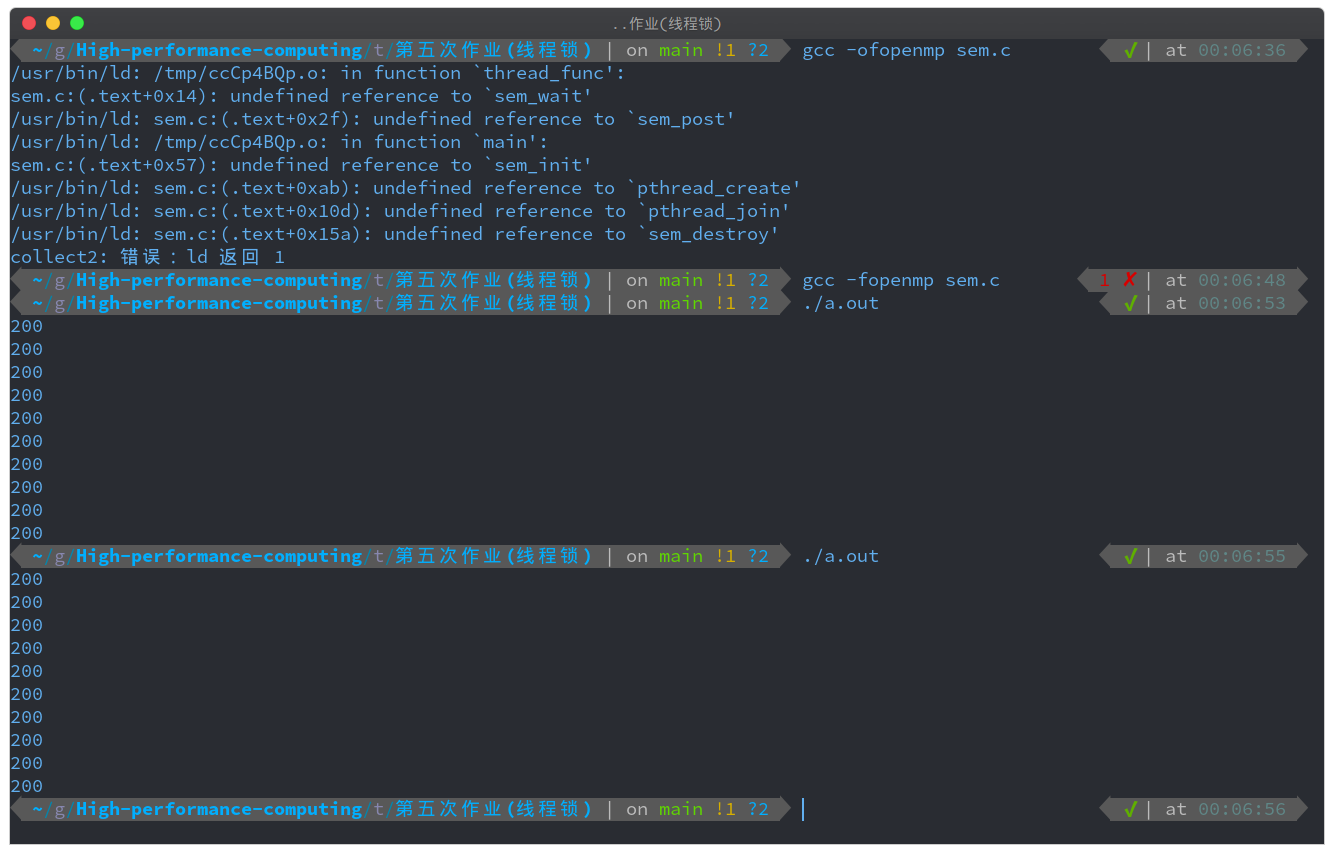
\includegraphics[scale=0.35]{../sem.png}
    \caption{信号量试验结果图}
    \label{sem}
\end{figure}

\section{读写锁}

\subsection{读写锁原理解析}

读写锁实将对共享资源的访问者划分成读者和写者,读者只对共享资源进行读访问,写者则需要对共享资源进行写操作。
一个读写锁同时只能有一个写者或多个读者,因为多个写者会造成结果混乱,且不能同时既有读者又有写者。

在写者需要修改共享资源时,需要加入读写锁;在对共享资源修改完毕后,需要释放读写锁(与互斥量的思想大体相同)。核心语法如下所示:

\begin{enumerate}
    \item {\ttfamily pthread\_rwlock\_t rwlock;} 创建读写锁;
    \item {\ttfamily pthread\_rwlock\_wrlock(\&rwlock);} 获取读写锁;
    \item {\ttfamily pthread\_rwlock\_unlock(\&rwlock);} 释放读写锁;
    \item {\ttfamily pthread\_rwlock\_destroy(\&rwlock);} 在不使用读写锁后,销毁读写锁。
\end{enumerate}

\begin{note}
    为方便结果展示,在读任务中也加入读写锁,即统一时刻只能有一个线程读取数据。否则打印读线程任务的结果时较为繁杂,不利于结果分析。
\end{note}

\subsection{读写锁实验流程与结果分析}

根据原理解析,创立两组线程和两个任务。第一个任务为写任务,负责{\ttfamily g\_Count++}操作;第二个任务为读任务,负责读取{\ttfamily g\_Count}的值。
第一组线程负责完成写任务,第二组线程负责完成读任务,并在读线程任务中打印{\ttfamily g\_Count}的值,以此来观察结果并分析。

在读线程任务中打印{\ttfamily g\_Count}的值,打印结果较多,不便使用截图展示。因此可执行文件的执行方式为{\ttfamily ./a.out > read\_write\_lock\_
result.txt}。因此,代码文件为提交作业中的{\ttfamily writeReadLock.c}文件,结果输出在{\ttfamily read\_write\_lock\_
result.txt}文件中。

创建20个线程,循环10次执行,截取其中一段结果:

\lstinputlisting[language=bash]{read_write.sh}

对给出的结果进行分析:
\begin{itemize}
    \item 1 线程获取读写锁,读取的变量是 17,读取完毕后释放读写锁;
    \item 2 线程获取读写锁,写完毕后释放读写锁;
    \item 3 线程获取读写锁,写完毕后释放读写锁;
    \item 4 线程获取读写锁,写完毕后释放读写锁;
    \item 5 线程获取读写锁,读取的变量是 20,读取完毕后释放读写锁;
    \item 打印出最后 count 的结果是20。
\end{itemize}


\section{条件变量}

\subsection{条件变量原理解析}

以生产者消费者模型为例说明条件变量的使用条件。为节省开销,希望生产者制造出 100 个产品后才通知消费者。
如果直接使用 mutex 互斥锁,需要在某个线程上不断地轮询:100 个产品是否生产完毕。
相当于进行大量无效的询问,才能知道条件是否已经满足,并且每次询问均需要加锁和释放锁,这无疑会带来额外的开销。
而条件变量则高效地解决了这个问题。使用条件变量的情况下,我们可以直接等待某个条件的发生,而不需要主动轮询。

条件变量是一种线程同步机制。核心思想是:一个线程等待“条件变量的条件成立”而挂起;另一个线程使“条件成立”。
为了防止竞争,条件的检测是在互斥锁的保护下进行的,线程在改变条件状态前先要锁住互斥量。

如果一个条件为假,则一个线程自动阻塞,该线程处于等待状态,并释放相关变量的互斥锁。
如果另一个线程改变了条件,它将信号发送给关联的条件变量,唤醒一个或多个处于等待中的线程,使其重新获得互斥锁,重新评价条件。

\begin{note}
由于{\ttfamily pthread\_cond\_signal}和{\ttfamily pthread\_cond\_broadcast}函数的调用都不需要加锁,
所以它们放到{\ttfamily pthread\_mutex\_unlock}之前或者之后执行都是可以的。
但在实际使用中,需要根据具体情况考虑它们的顺序,来使得程序高效运行。

当{\ttfamily signal}操作发生在{\ttfamily unlock}之前时,其他等待的线程被唤醒,但{\ttfamily signal}锁可能仍然没有释放,
导致被唤醒的线程无法获取到{\ttfamily mutex}锁,从而再次进入休眠。通常情况下,这种调用顺序就会对代码的执行效率产生不良的影响。
\end{note}

核心语法如下所示:
\begin{enumerate}
    \item {\ttfamily pthread\_cond\_t cond = PTHREAD\_COND\_INITIALIZER;} 初始换条件变量;
    \item {\ttfamily pthread\_cond\_signal(\&cond);} 完成某任务后,条件变量发射信号;
    \item {\ttfamily pthread\_cond\_wait(\&cond, \&mutex);} 位于条件判断语句后,若条件成立,线程阻塞处于等待状态,并释放互斥锁;
    \item {\ttfamily pthread\_cond\_destroy(\&cond);} 销毁条件变量。
\end{enumerate}

\begin{note}
但由于系统实现,会存在虚假唤醒等情况。即:线程并没有发出通过{\ttfamily pthread\_cond\_signal}或{\ttfamily pthread\_cond\_broadcast}
发出唤醒信号,处于等待中的线程仍然会自己醒来,这是一种能保证执行效率的方法。

假设此时有10个线程处于等待中,在收到一个唤醒信号后,操作系统尝试去唤醒所有的线程,这会打破发送信号与唤醒之间一对一的关系。
所以此时只能唤醒一个线程,而其余九个线程处于等待阶段。为了更灵活的处理这种情况,所以无论条件是否满足,
操作系统允许等待中的线程自己醒来,称为虚假唤醒。

为了避免虚假唤醒对条件带来的影响,条件判断需要使用{\ttfamily while}而不是{\ttfamily if}。这是由于 wait 函数被唤醒时,
存在虚假唤醒等情况,导致唤醒后发现条件依旧不成立。因此需要使用{\ttfamily while}语句来循环地进行等待,直到条件成立为止。
\end{note}

\subsection{条件变量实验流程与结果分析}

根据原理解析中生产者与消费者的模型,创建100个线程,且每当{\ttfamily count \% 20 == 0}时叫醒等待中的线程,
防止过度轮循。试验结果如图\ref{cond}所示,代码文件为提交作业中的{\ttfamily conVar.c}。

\begin{figure}[h]
    \centering
    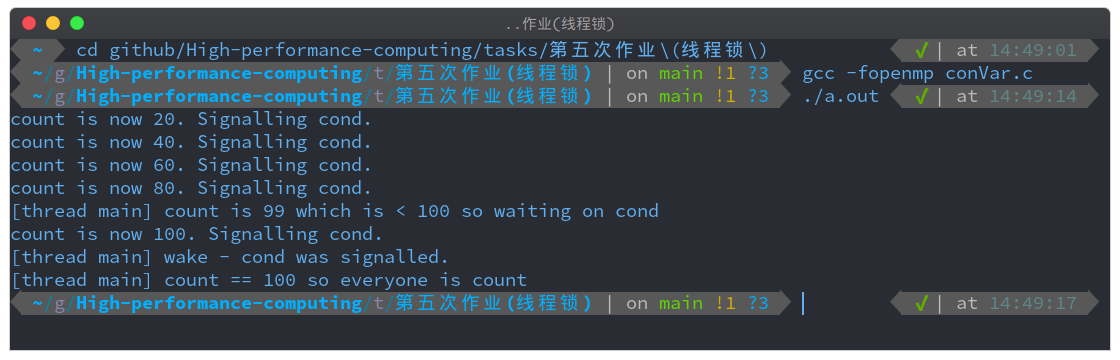
\includegraphics[scale=0.35]{../cond.png}
    \caption{条件变量试验结果图}
    \label{cond}
\end{figure}

在图\ref{cond}中,可以观察到,在{\ttfamily count}取值为20,40,60,80时,由于{\ttfamily signal}叫醒速度过快,等待线程没有及
时获取{\ttfamily mutex}锁来响应,因此等待线程中没有任何输出。而当等待线程因为虚假唤醒判断条件是否满足时,因为99小于100,
不满足条件,所以等待线程继续等待。当最后{\ttfamily count}的取值为100时,等待线程被唤醒并继续向后执行,打印
{\ttfamily [thread main] wake - cond was signalled.}语句,在程序的极为,打印出最后的输出语句来
判断{\ttfamily count}的值是否正确,结果{\ttfamily [thread main] count == 100 so everyone is count}显示答案正确。

\end{document}